\documentclass[border=10pt]{standalone}

\usepackage{tikz}
\usepackage{tikzsymbols}
\usetikzlibrary{calc,patterns,shapes.geometric}

\def\centerarc[#1](#2)(#3:#4:#5){\draw[#1] ($(#2)+({#5*cos(#3)},{#5*sin(#3)})$) arc (#3:#4:#5);}

\begin{document}
	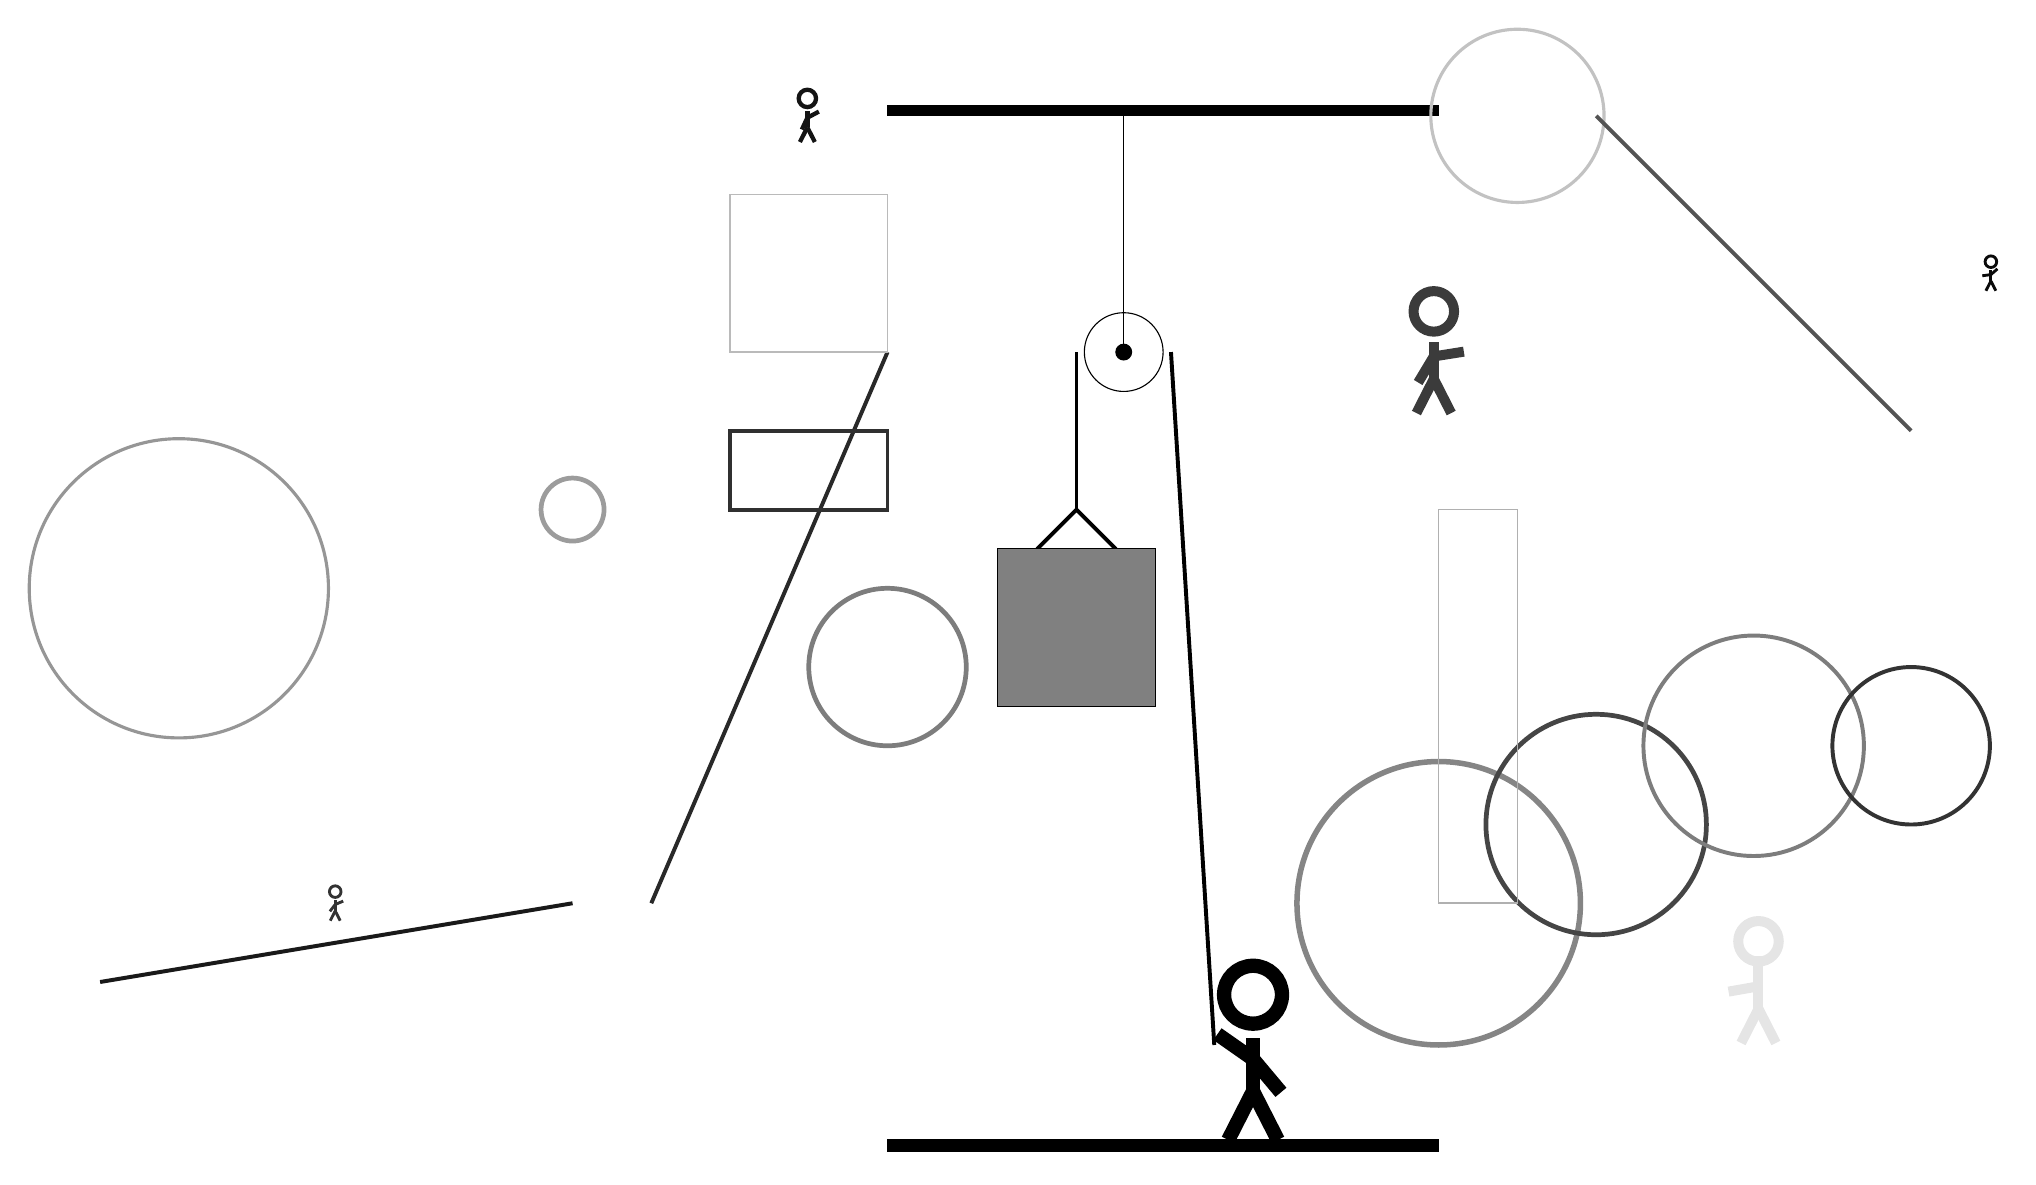
\begin{tikzpicture}
		%%%%% START %%%%%
		
		\draw[fill=black] (-2, 10) rectangle (5, 10.125);
		
		\draw[line width=0.5mm, color=black!84](-5, 0) -- (-2, 7);
		
		\draw [line width=0.6mm, color=black!39](-6, 5) circle (0.4);
		\draw [line width=0.4mm, color=black!24](6, 10) circle (1.1);
		\draw [line width=0.7mm, color=black!48](5, 0) circle (1.8);
		\draw [line width=0.6mm, color=black!73](7, 1) circle (1.4);
		\draw [line width=0.6mm, color=black!51](-2, 3) circle (1.0);
		\node[line width=0.2mm, color=black!96] at (12, 8) {\Strichmaxerl[2][8][41]};
		\draw[line width=0.2mm, color=black!31] (6, 5) rectangle (5, 0);
		\draw [line width=0.4mm, color=black!41](-11, 4) circle (1.9);
		\node[line width=0.2mm, color=black!80] at (-9, 0) {\Strichmaxerl[2][52][23]};
		\draw [line width=0.5mm, color=black!51](9, 2) circle (1.4);
		\draw[line width=0.5mm, color=black!81] (-4, 5) rectangle (-2, 6);
		\draw[line width=0.5mm, color=black!90](-6, 0) -- (-12, -1);
		\draw[line width=0.2mm, color=black!27] (-2, 7) rectangle (-4, 9);
		\draw [line width=0.5mm, color=black!80](11, 2) circle (1.0);
		\node[line width=0.5mm, color=black!77] at (5, 7) {\Strichmaxerl[7][59][9]};
		\node[line width=0.7mm, color=black!92] at (-3, 10) {\Strichmaxerl[3][65][28]};
		
		\draw[line width=0.5mm, color=black!67](7, 10) -- (11, 6);
		\node[line width=0.7mm, color=black!10] at (9, -1) {\Strichmaxerl[7][10][90]};
		
		\draw (1, 7) circle (0.5);
		\draw[fill=black] (1, 7) circle (0.1);
		\draw (1, 10) -- (1, 7);
		
		\draw[line width=0.5mm] (-0.1, 4.5) -- (0.4, 5.0) -- (0.9, 4.5);
		\draw[fill=black!50] (-0.6, 4.5) rectangle (1.4, 2.5);
		
		\draw[line width=0.5mm] (0.4, 7) -- (0.4, 5.0);
		\centerarc[line width=0.5mm](1, 7)(0:180:0.6);
		\draw[line width=0.5mm](1.6, 7) -- (2.15, -1.8);
		
		\node at (2.6, -1.9) {\Strichmaxerl[10][-35][-50]};
		
		\draw[fill=black] (-2, -3) rectangle (5, -3.15);
		
		%%%%% END %%%%%
	\end{tikzpicture}
\end{document}